% Created 2014-03-14 Fri 08:33
\documentclass[11pt]{article}
\usepackage[utf8]{inputenc}
\usepackage[T1]{fontenc}
\usepackage{fixltx2e}
\usepackage{graphicx}
\usepackage{longtable}
\usepackage{float}
\usepackage{wrapfig}
\usepackage{soul}
\usepackage{textcomp}
\usepackage{marvosym}
\usepackage{wasysym}
\usepackage{latexsym}
\usepackage{amssymb}
\usepackage{hyperref}
\tolerance=1000
\usepackage{xeCJK}
\setCJKmainfont{SimSun}
\usepackage{xeCJK}
\setCJKmainfont{SimSun}
\providecommand{\alert}[1]{\textbf{#1}}

\title{emacs}
\author{xwp}
\date{\today}
\hypersetup{
  pdfkeywords={},
  pdfsubject={},
  pdfcreator={Emacs Org-mode version 7.8.11}}

\begin{document}

\maketitle

\setcounter{tocdepth}{3}
\tableofcontents
\vspace*{1cm}
\section{Emacs和vim}
\label{sec-1}
\subsection{影响力}
\label{sec-1-1}

   vim是编辑器之神,打字速度飞快,当熟练后,手比脑快;
   Emacs是神的编辑器,功能强大,可扩展性极强,是IT大神和黑客们御用编辑器,是GNU创始人Richard Stallman的作品,
   据说Google和苹果里很多工程师在使用。
\subsection{使用感受}
\label{sec-1-2}

   vim,已使用7年有余,一个字形容,“爽”,敲代码非常过瘾,启动速度快,但像有的网友描述的那样,vim用久了
   感觉我的性子变急了。

   Emacs,断断续续使用3年有余,但一直停留在初级水平,学习曲线真的很陡,往往使用上十天半个月,遇到不会使用的
   模式或快捷键,不自觉的又去用vim解决问题,不过Emacs真心强大,我知道这会是我的最终选择,终身伴侣。
   这次借整理博客之际,决定彻底加入Emacs阵营,已经把vi/vim alias emacs。
\section{安装Emacs24}
\label{sec-2}


\begin{verbatim}
1.去emcse官网下载emacs24源码包
2.sudo apt-get install build-essential
sudo apt-get build-dep emacs23
3.cd  src-emacs
./configure
make
sudo make install
\end{verbatim}
\section{Emacs工作原理和模式}
\label{sec-3}
\subsection{模式}
\label{sec-3-1}
\subsubsection{major-mode模式}
\label{sec-3-1-1}

\begin{itemize}
\item 符号——即用来实现这个模式的函数名
\item 名字——这个主编辑模式显示在状态栏里的名称
\item 局部键位图——用来定义这个主编辑模式下各种命令的按键绑定
\item 变量和常数——为了实现这个主编辑模式,LISP需要使用的一些局部变量和局部常数
\item 专用编辑缓冲区——这个主编辑模式下有特殊用途的编辑缓冲区
\end{itemize}
\subsubsection{mode-hooks模式}
\label{sec-3-1-2}

    也是又LISP编写的代码,当修改某一主模式时,可让主模式加载挂钩模式,实现主模式的扩展,挂钩模式里的变量或按键
    绑定可以覆盖掉主模式里的内容。一个主模式可以添加多个挂钩模式。
\section{Emacs基本操作}
\label{sec-4}

  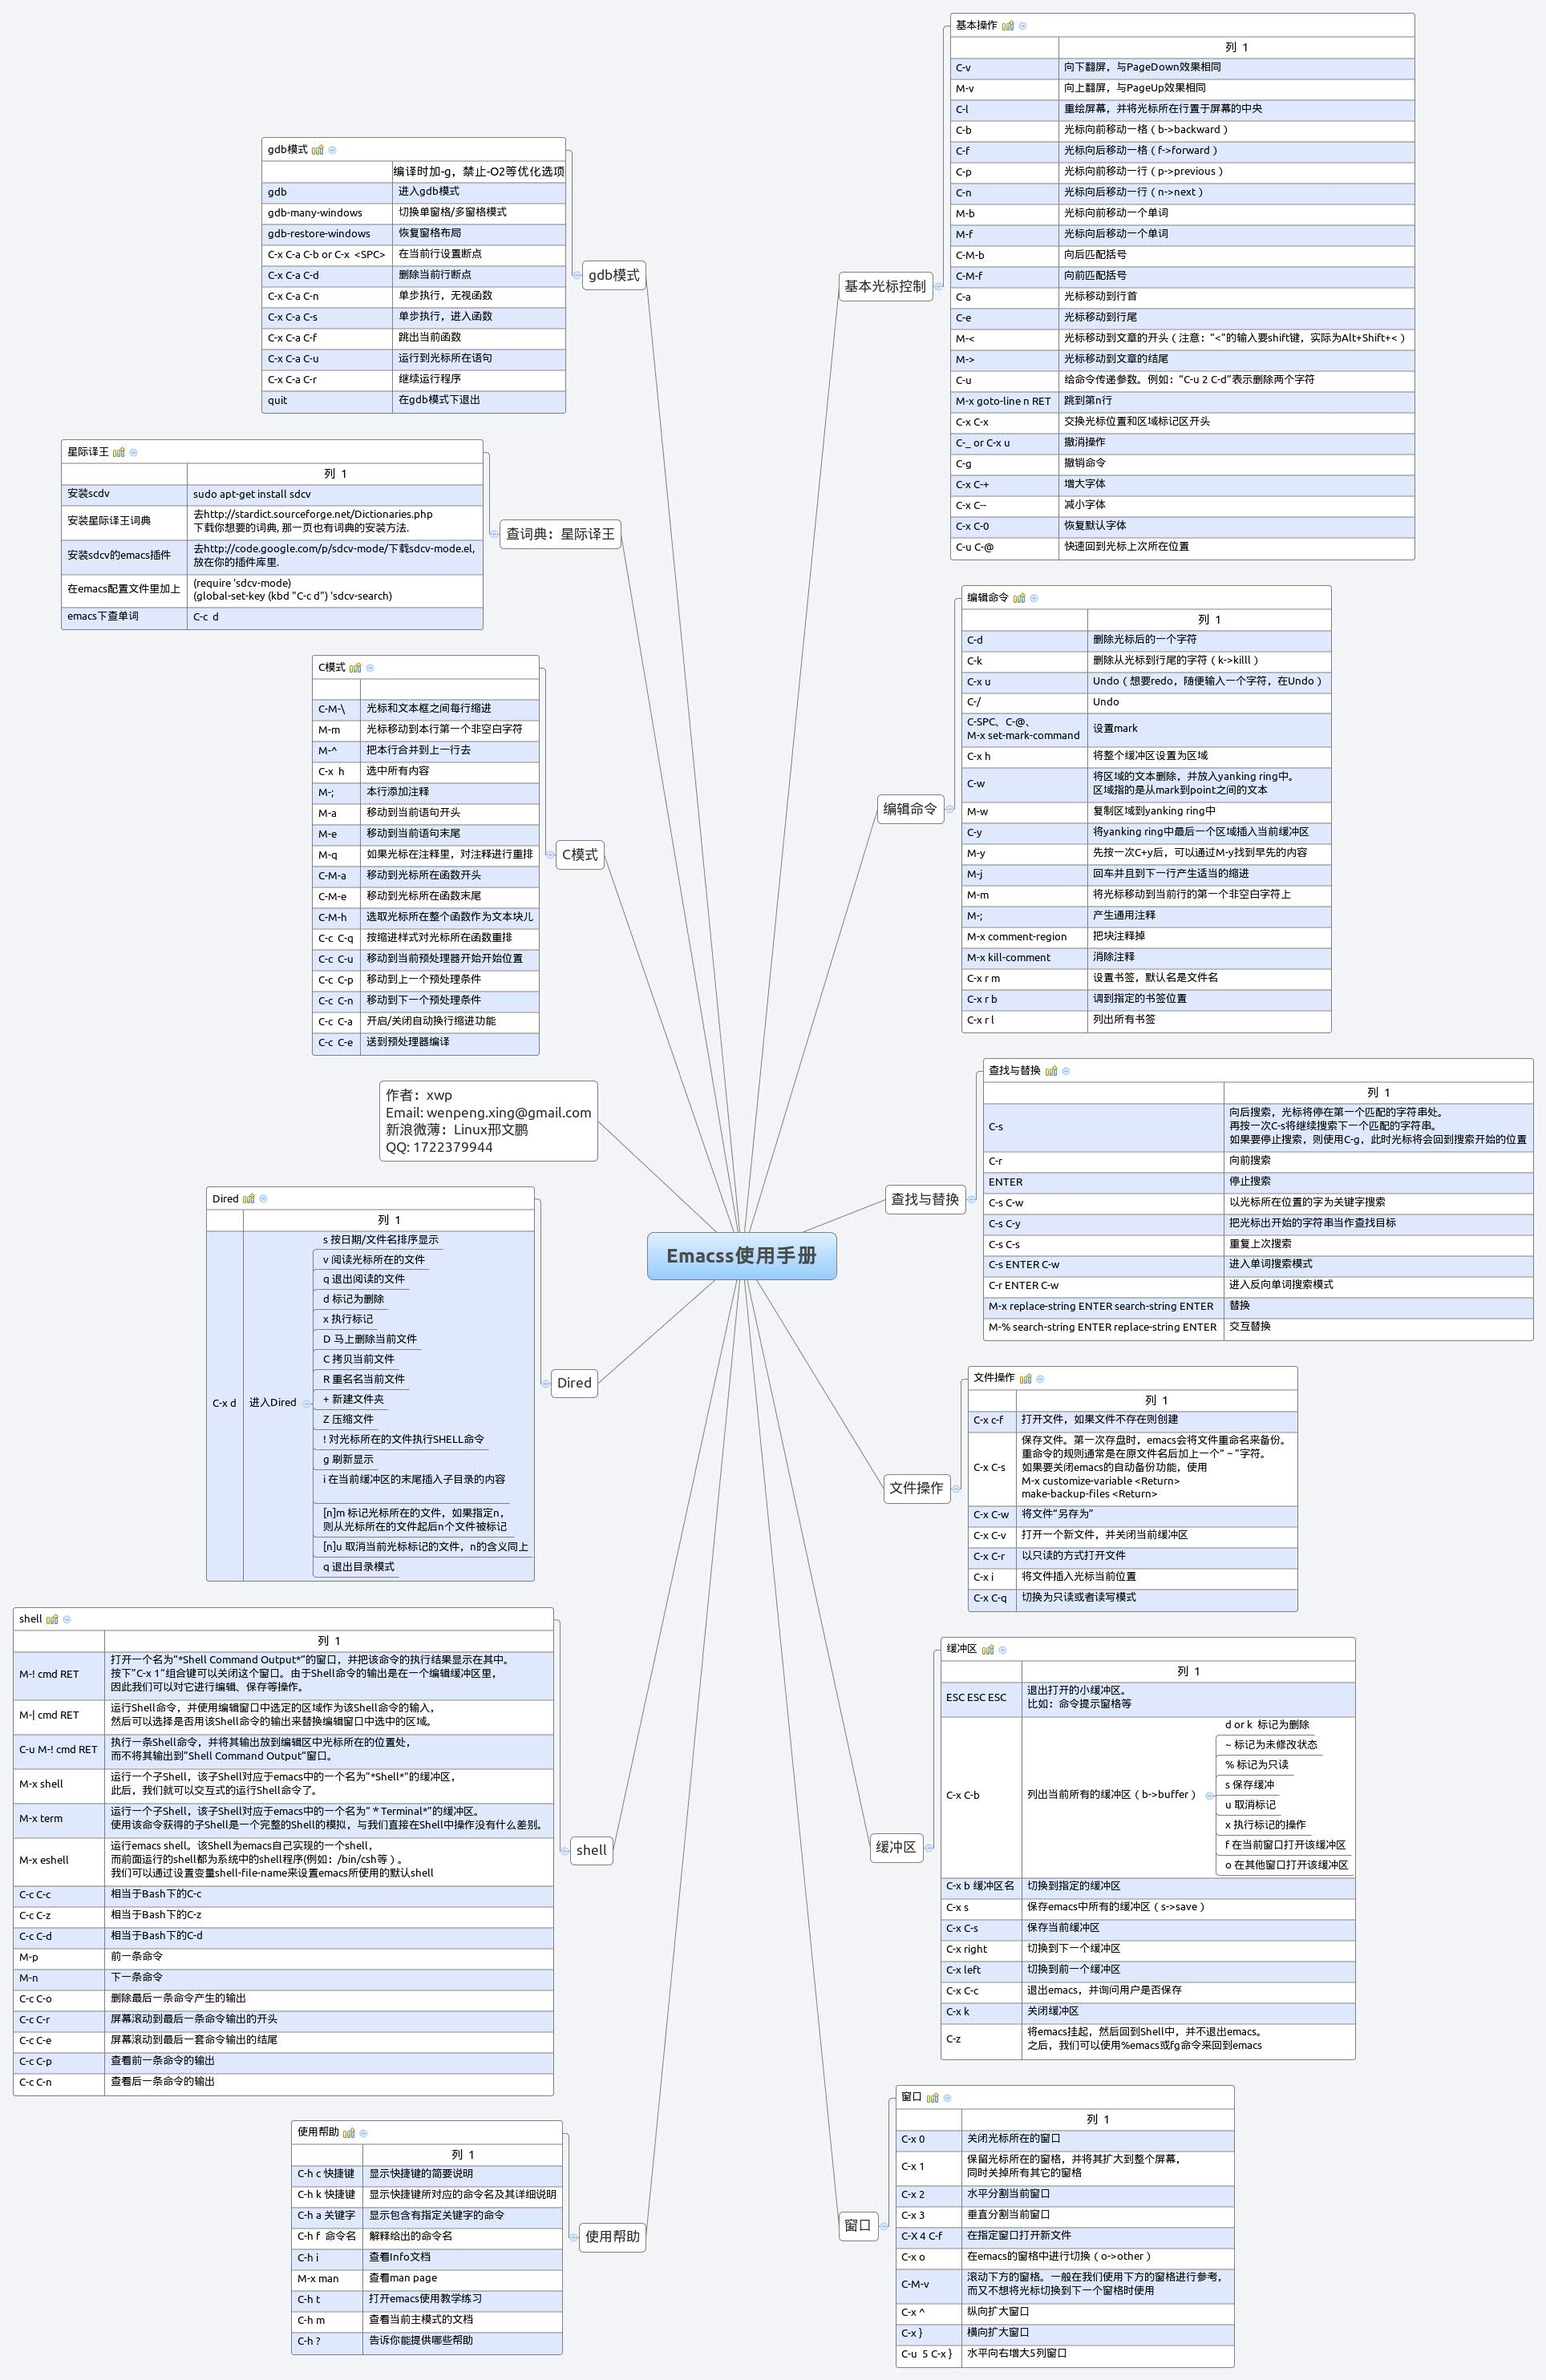
\includegraphics[width=.9\linewidth]{./images/Emacs-base.jpg}
\section{站在巨人肩膀上使用Emacs}
\label{sec-5}

  我参照的是陈斌的emacs设置,他的文章写的很好,我受益颇多\href{http://blog.csdn.net/redguardtoo/article/details/7222501}{一年成为Emacs高手(像神一样使用编辑器)}
  ,作为Emacs初级水平,还是以读懂和模仿高手的Emacs配置为主,中国人最擅长的也是模仿,消化吸收,再创新。不要一开始纠结于自己去定制
  自己Emacs环境,那样你会走向我曾走过的弯路,3年都没有真正上手。
\section{Emacs之org模式}
\label{sec-6}
\subsection{安装org}
\label{sec-6-1}

\begin{enumerate}
\item 在emacs中更新org mode版本

   M+x list-packages

   找到org,大I,表示安装
\item 为org mode 输出pdf做设置,编辑\~{}/.emacs文件,加入下面设置,注意你的org-mode版本,如果是刚更新过的org mode选用org mode 8.0那行代码。

\begin{verbatim}


;; org-mode < 8.0
(setq org-latex-to-pdf-process '("xelatex -interaction nonstopmode %f"
"xelatex -interaction nonstopmode %f"))
;;  org-mode 8.0
(setq org-latex-pdf-process '("xelatex -interaction nonstopmode %f"
"xelatex -interaction nonstopmode %f"))
\end{verbatim}

   3.此时可以先测试下org mode 是否可以输出pdf文件了

   4.添加pdf输出中文支持

   将C:/windows/fonts下你喜欢的字体拷贝到/usr/share/fonts/windows目录下(需首先创建windows目录)

   然后将对应字体拷贝到该目录下(需使用管理员权限sudo执行,我拷贝的是常用的六种中文字体simsun.ttc 和sim开头的.ttf) 

   加载字库文件时需要有读权限

   suod chmod 644 /usr/share/fonts/windows/*

   5.生成ubuntu下的字库索引

\begin{verbatim}
cd /usr/share/fonts/windows
sudo mkfontscale  
sudo mkfontdir  
sudo fc-cache -fv
\end{verbatim}

   6.注销系统

   7.查看是否生成了中文字体支持

   fc-list :lang=zh

   8.在你写file.org文件开头添加


\begin{verbatim}
#+LATEX_HEADER: \usepackage{xeCJK}
#+LATEX_HEADER: \setCJKmainfont{SimSun}
\end{verbatim}
\end{enumerate}
\subsection{基本操作}
\label{sec-6-2}
\subsubsection{定义标题}
\label{sec-6-2-1}

    用emacs新建test.org

\begin{verbatim}
*一级标题
正文
**二级标题
正文
***三级标题
正文
依次类推,最多十级标题
\end{verbatim}


\begin{center}
\begin{tabular}{ll}
 快捷键          &  命令说明                                  \\
\hline
 S-Tab           &  循环三种状态,折叠,打开下一级,全部打开  \\
 Tab             &  循环切换光标所在大纲状态                  \\
 C-c C-n/p       &  上/下一标题                               \\
 C-c C-f/b       &  上/下一标题(仅限同一标题)               \\
 M-RET           &  插入同一级标题                            \\
 M-S-RET         &  插入同一级todo标题                        \\
 M-left/right    &  将同一级标题升级/降级                     \\
 M-S-left/right  &  将当前标题子树升级/降级                   \\
 M-up/down       &  将当前标题上移/下移                       \\
 M-S-up/down     &  将当前标题子树上移/下移                   \\
 C-c *           &  将本行设为标题/正文                       \\
 C-c C-w         &  将子树或区域移动到另一标题处(跨缓冲区)  \\
\end{tabular}
\end{center}


    
\subsubsection{轻量标记语言}
\label{sec-6-2-2}
\begin{itemize}

\item 字体\\
\label{sec-6-2-2-1}%
\begin{verbatim}
*粗体*
/斜体/
+删除线+
_下划线_
下标: H_2 O
上标: E=mc^2
等宽字:  =git=  或者 ~git~
\end{verbatim}

\item 表格\\
\label{sec-6-2-2-2}%
\begin{center}
\begin{tabular}{ll}
 快捷键        &  命令解释                      \\
\hline
 C-c 竖线      &  创建表格                      \\
 C-c C-c       &  对齐表格                      \\
 Tab           &  移动下一区域                  \\
 S-Tab         &  移动到上一区域                \\
 RET           &  移动到下一行,必要时新建一行  \\
 M-left/right  &  移动列                        \\
 M-up/down     &  移动行                        \\
 M-S-left      &  删除当前列                    \\
 M-S-right     &  向前插入列                    \\
 M-S-up        &  删除当前行                    \\
 M-S-down      &  向上插入行                    \\
 C-c \^{}      &  根据当前列排序                \\
\end{tabular}
\end{center}



\item 段落\\
\label{sec-6-2-2-3}%
对于单个回车换行的文本,认为其属于同一个段落。在导出的时候将会转化为不换行的同一段。如果要新起一个段落,需要留出一个空行。

\item 列表\\
\label{sec-6-2-2-4}%
Org 能够识别有序列表、无序列表和描述列表。

\begin{verbatim}
+ 无序列表项以 - 、=+= 或者 * 开头。
+ 有序列表项以 1. 或者 1) 开头。
\end{verbatim}

\item 分割线\\
\label{sec-6-2-2-5}%
5条短线或以上,显示为分割线

\begin{verbatim}
-----
\end{verbatim}

\end{itemize} % ends low level
\subsubsection{发布准备工作}
\label{sec-6-2-3}
\begin{itemize}

\item 文档元数据\\
\label{sec-6-2-3-1}%
\begin{verbatim}
#+TITLE:       the title to be shown (default is the buffer name)
#+AUTHOR:      the author (default taken from user-full-name)
#+DATE:        a date, an Org timestamp1, or a format string for format-time-string
#+EMAIL:       his/her email address (default from user-mail-address)
#+DESCRIPTION: the page description, e.g. for the XHTML meta tag
#+KEYWORDS:    the page keywords, e.g. for the XHTML meta tag
#+LANGUAGE:    language for HTML, e.g. ‘en’ (org-export-default-language)
#+TEXT:        Some descriptive text to be inserted at the beginning.
#+TEXT:        Several lines may be given.
#+OPTIONS:     H:2 num:t toc:t \n:nil @:t ::t |:t ^:t f:t TeX:t ...
#+BIND:        lisp-var lisp-val, e.g.: org-export-latex-low-levels itemize
         You need to confirm using these, or configure org-export-allow-BIND
#+LINK_UP:     the ``up'' link of an exported page
#+LINK_HOME:   the ``home'' link of an exported page
#+LATEX_HEADER: extra line(s) for the LaTeX header, like \usepackage{xyz}
#+EXPORT_SELECT_TAGS:   Tags that select a tree for export
#+EXPORT_EXCLUDE_TAGS:  Tags that exclude a tree from export
#+XSLT:        the XSLT stylesheet used by DocBook exporter to generate FO file
\end{verbatim}
     其中\#+OPTIONS是复合的选项,包括:

\begin{verbatim}
H:         set the number of headline levels for export
num:       turn on/off section-numbers
toc:       turn on/off table of contents, or set level limit (integer)
\n:        turn on/off line-break-preservation (DOES NOT WORK)
@:         turn on/off quoted HTML tags
::         turn on/off fixed-width sections
|:         turn on/off tables
^:         turn on/off TeX-like syntax for sub- and superscripts.  If
     you write "^:{}", a_{b} will be interpreted, but
     the simple a_b will be left as it is.
-:         turn on/off conversion of special strings.
f:         turn on/off footnotes like this[1].
todo:      turn on/off inclusion of TODO keywords into exported text
tasks:     turn on/off inclusion of tasks (TODO items), can be nil to remove
     all tasks, todo to remove DONE tasks, or list of kwds to keep
pri:       turn on/off priority cookies
tags:      turn on/off inclusion of tags, may also be not-in-toc
<:         turn on/off inclusion of any time/date stamps like DEADLINES
*:         turn on/off emphasized text (bold, italic, underlined)
TeX:       turn on/off simple TeX macros in plain text
LaTeX:     configure export of LaTeX fragments.  Default auto
skip:      turn on/off skipping the text before the first heading
author:    turn on/off inclusion of author name/email into exported file
email:     turn on/off inclusion of author email into exported file
creator:   turn on/off inclusion of creator info into exported file
timestamp: turn on/off inclusion creation time into exported file
d:         turn on/off inclusion of drawers
\end{verbatim}
     这些元数据可以根据需要设置。建议放在文档的开头部分。如,本文采用的元数据如下:

\begin{verbatim}
#+TITLE: org-mode
#+AUTHOR:xingwenpeng
#+EMAIL: wenpeng.xing@gmail.com
#+KEYWORDS: emacs, org-mode
#+OPTIONS: H:4 toc:t
\end{verbatim}

\item 内容元数据\\
\label{sec-6-2-3-2}%
分行区块,默认内容不换行,需要留出空行才能换行。定义了分行的区块可以实现普通换行:

\begin{verbatim}
\begin{verse}
Great clouds overhead\\textbackslash{}
Tiny black birds rise and fall\\textbackslash{}
Snow covers Emacs\\textbackslash{}
-- AlexSchroeder\\
\end{verse}

\end{verbatim}
      引用区块,通常用于引用,与默认格式相比左右都会留出缩进:

\begin{verbatim}
\begin{quote}
缩进区块
\end{quote}

\end{verbatim}

      居中区块

\begin{verbatim}
\begin{center}
Everything should be made as simple as possible, \\
but not any simpler
\end{center}

\end{verbatim}

      代码区块

\begin{verbatim}
    #+BEGIN_SRC ruby
require 'redcarpet'
md = Redcarpet.new("Hello, world.")
puts md.to_html
    #+END_SRC
\end{verbatim}

      例子

\begin{verbatim}
: 单行的例子以冒号开头

      :#+BEGIN_EXAMPLE
      多行的例子
      使用区块
      :#+END_EXAMPLE
\end{verbatim}

\item 导出
\label{sec-6-2-3-3}%
\begin{verbatim}
 C-c C-e
\end{verbatim}
如果想导出PDF并支持中文,当前环境中需安装中文ttf字库,并在org文件开头添加

\begin{verbatim}
#+LATEX_HEADER: \usepackage{xeCJK}
#+LATEX_HEADER: \setCJKmainfont{SimSun}
\end{verbatim}

\end{itemize} % ends low level
\section{org实现GTD}
\label{sec-7}
\subsection{todo模式}
\label{sec-7-1}
\subsubsection{\textbf{TODO} test    \textit{2014-03-12 Wed}--\textit{2014-04-12 Sat}}
\label{sec-7-1-1}

qdsfadsf
\subsubsection{\textbf{DONE} abdcsdf}
\label{sec-7-1-2}

    \texttt{SCHEDULED:} \textit{2014-03-12 Wed}

\begin{itemize}
\item State ``DONE''       from ``STARTED''    \textit{2014-03-12 Wed 16:02}
\end{itemize}
\textit{2014-03-12 Wed}
sdfadflksfd
\subsection{文件设置}
\label{sec-7-2}
\subsubsection{设置org-agenda监控文件,如:}
\label{sec-7-2-1}


\begin{verbatim}
(setq org-agenda-files (list "~/org/linux.org"
                   "~/org/work.org"
                   "~/org/home.org"))
\end{verbatim}
\subsubsection{设置org内置tag}
\label{sec-7-2-2}


\begin{verbatim}
(setq org-tag-alist '(("苦差" . ?k)
                            ("薪水" . ?s)))
\end{verbatim}
\subsubsection{设置按tag查看的快捷命令}
\label{sec-7-2-3}

      这段代码表示您定了一个可以用C-c a k 调出来的view,它的描述是”work haha”,view中包含三段数据。
      最上面是agenda,就是调C-c a a出来的界面,然后一个分隔行,列出tags为“work”的项目,再一个分隔行,列出tags为支持的项目。

\begin{verbatim}
(setq org-agenda-custom-commands
'(("k" "work haha"
((agenda "")
(tags-todo "work")
(tags-todo "支持")))))
\end{verbatim}
\subsubsection{设置remember快捷键}
\label{sec-7-2-4}

    remember是随时需要的东西,用完后又应该随时忘掉。所以调用remember应该越不影响当前的思路又好。
    一个要键入”M-x org-remember”这么多字符才能调出来的remember又有什么用?然后“C-c C-c”保存(C-c C-k是取消),
    remember buffer自动消失,整个emacs又恢复成写这篇org的界面。

\begin{verbatim}
(define-key global-map [f12] 'org-remember)
\end{verbatim}
\subsubsection{加载变量设置}
\label{sec-7-2-5}

    我的Emacs初始化文件.emacs会加载当前机器设置的变量,所以我把设置监控文件和tag语句放到了.custom.el中

\begin{verbatim}
(if (file-readable-p (expand-file-name "~/.custom.el"))
    (load-file (expand-file-name "~/.custom.el")))
\end{verbatim}
    
\subsection{基本操作}
\label{sec-7-3}


\begin{center}
\begin{tabular}{ll}
 快捷键          &  命令解释                           \\
\hline
 C-S-RET         &  创建*开头的TODO                    \\
 C-c C-s         &  选定调度时间                       \\
 C-c C-t         &  选择改变TODO状态                   \\
 S-left/right    &  循环改变TODO状态                   \\
 S-M-left/right  &  改变TODO条目的大纲级别,层级改变   \\
 C-c a t         &  显示全局TODO条目                   \\
 C-c C-t         &  选定截止时间                       \\
 C-c C-x C-i     &  开始计时                           \\
 C-c C-x C-o     &  结束计时                           \\
 C-c C-q         &  打标签                             \\
 C-c a m         &  按标签索引被监控的文件             \\
 C-c C-x a       &  将节点打上achived标签              \\
 C-c C-x A       &  将当前节点归入名为Archive的子树中  \\
\end{tabular}
\end{center}


   
\subsubsection{\textbf{DONE} 时间设定 \textbf{:home:}}
\label{sec-7-3-1}

    \texttt{CLOSED:} \textit{2014-03-13 Thu 11:34}

\begin{itemize}
\item State ``DONE''       from ``''           \textit{2014-03-13 Thu 11:34}
\end{itemize}
    \#+begin$_{\mathrm{exmaple}}$
    \textit{2014-03-13 Thu .+1m} 
    \texttt{SCHEDULED:} \textit{2014-04-13 Sun .+1m}

\begin{itemize}
\item State ``DONE''       from ``TODO''       \textit{2014-03-13 Thu 11:01}
    日期repeater标记分为日(d),周(w),月(m),年(y)四种,后面的.+1m代表这一任务在每月循环一次,当你用C-c C-t改变Item状态之后,这个项目并不会从TODO变成DONE,而是保持TODO状态,同时它的DEADLINE从03-13变成04-13,下面出现一个3-13的CLOSING NOTE,表示这个项目在12月26日被标记为DONE过。
\end{itemize}

    \#+end$_{\mathrm{exmaple}}$
    
\subsection{标签}
\label{sec-7-4}
\subsection{分类}
\label{sec-7-5}
\subsection{归档}
\label{sec-7-6}

   如果你用org-mode来做TODO管理,那么无法避免的是,随着时间的流逝,被DONE的事件会越来越多,那么TODO被会被夹杂在DONE之间,难以查找。同时,由于后期回顾的需要,你也不想简单地将DONE事件删除掉。这个时候,你就需要归档命令了。归档,就是把你不想天天看到的东西,放到你看不到了,或者不怎么影响你的注意力的地方去。org-mode提供了两种归档方式。
\subsubsection{内部归档}
\label{sec-7-6-1}

    内部归档是在本文件内部给特定子树打上ACHIVED标签或者移动到名为achived的子树中去并打上标签。

\begin{verbatim}
C-c C-x a
将某一个节点打上ARCHIVE标签。
C-c C-x A
将当前节点归入一个名为Archive的子树中,并且这个子树是位于当前级别子树的最下方。
\end{verbatim}
\subsubsection{外部归档}
\label{sec-7-6-2}

    外部归档是指把子树移动到另一个org文件中去。文件名可以自定义。默认情况下,归档的子树会被移动到名为“当年文件名$_{\mathrm{archived}}$”的文件中去。
    

\begin{verbatim}
C-c C-x C-s是把当前的节点移到archived文件中去。
我个人还是更喜欢在文件内部做归档。因为它兼具归档的好处和查找的方便。
在任何一个树的子树中,只有一个archive子树,只占文档的一行,当你居然查看以前存档的事件时,只能在这个节点上使用”C-TAB”命令即可打开。
\end{verbatim}
\section{Emacs之w3m模式}
\label{sec-8}
\subsection{快捷键}
\label{sec-8-1}


\begin{center}
\begin{tabular}{ll}
 快捷键       &  命令解释                   \\
\hline
 D            &  下载此URL                  \\
 E            &  编辑此URL                  \\
 F            &  前往行                     \\
 M            &  外部查看                   \\
 Y            &  打印当前URL                \\
 M-i          &  保存图片                   \\
 M-2          &  切换窗口到2                \\
 C-a          &  到行首                     \\
 C-e          &  到行尾                     \\
 C-l          &  当前行到中间               \\
 RET          &  打开当前链接               \\
 SPC          &  下翻一屏                   \\
 .            &  到网页最开头               \\
 =            &  查看html头                 \\
 G            &  在新会话中打开URL          \\
 H            &  主页                       \\
 Q            &  退出w3m                    \\
 R            &  重新加载此页               \\
 S            &  在新会话中显示搜索结果     \\
 l            &  返回上一页                 \\
 n            &  查看下一页                 \\
 o            &  查看历史                   \\
 q            &  关闭窗口                   \\
 C-c C-k      &  暂停打开网页               \\
 C-c C-n      &  移动到下一个会话           \\
 C-c C-p      &  移动到上一个会话           \\
 C-c C-s      &  选择会话                   \\
 C-t R        &  从新加载所有页面           \\
 M-s          &  选择会话                   \\
 C-c C-x C-w  &  org-w3m-copy-for-org-mode  \\
 C-c C-w      &  关闭当前会话               \\
 C-u S        &  选择使用哪种搜索引擎       \\
\end{tabular}
\end{center}
\subsection{设置默认搜索引擎}
\label{sec-8-2}

   修改.emacs.d目录下init-emacs-w3m.el文件
\section{Emacs之gdb模式}
\label{sec-9}
\section{Emacs之evil模式}
\label{sec-10}
\section{Emacs之etags阅读代码}
\label{sec-11}
\subsection{生成TAGS}
\label{sec-11-1}


\begin{verbatim}
find . -name "*.[chCHS]" | etags -
\end{verbatim}
\subsection{代码查看快捷键}
\label{sec-11-2}

   进入emacs,M-x visit-tag-table,选择刚生成的TAGS文件,即可开始emacs导游的源码之旅。

\begin{center}
\begin{tabular}{ll}
 快捷键   &  命令解释            \\
\hline
 C-]      &  查看光标处函数定义  \\
 C-t      &  从函数定义处返回    \\
 C-M-.    &  查找函数定义        \\
 M-.      &  查看光标处函数定义  \\
 M-*      &  回退                \\
 C-u M-.  &  查找标签的下一定义  \\
\end{tabular}
\end{center}
\section{vim简介}
\label{sec-12}

  Vim是从 vi 发展出来的一个文本编辑器。代码补完、编译及错误跳转等方便编程的功能特别丰富,在程序员中被广泛使用。和Emacs并列成为类Unix系统用户最喜欢的编辑器。
  使用vim先知道其设计理念是很重要的,有助于记忆,举一反三;
\subsection{vim的设计理念是组合;}
\label{sec-12-1}

   命令组合: Vim强大的编辑能力中很大部分是来自于其普通模式命令。vim的设计理念是命令的组合。例如普通模式命令''dd''删除当前行,''dj''代表删除到下一行,原理是第一个''d''含义是删除,''j''键代表移动到下一行,组合后''dj''删除当前行和下一行。另外还可以指定命令重复次数,''2dd''(重复''dd''两次),和''dj''的效果是一样的。''d^'',''^''代表行首,故组合后含义是删除到光标开始到行首间的内容(不包含光标);''d\$'' \$''代表行尾,删除到行尾的内容(包含光标);用户学习了各种各样的文本间移动/跳转的命令和其他的普通模式的编辑命令,并且能够灵活组合使用的话,能够比那些没有模式的编辑器更加高效的进行文本编辑。
   模式间的组合: 在普通模式中,有很多方法可以进入插入模式。比较普通的方式是按''a''(append/追加)键或者''i''(insert/插入)键。
\subsection{vim针对程序语言代码编写者;}
\label{sec-12-2}

   写代码的时候手需要时刻保持在键盘上,随机定位代码、随机删除代码、移动代码、插入代码的操作大大多于阅读、翻页操作,中间卡顿一下效率就大大降低了;但对普通用户而言,顺序写、设置字体格式、翻页读多于随机写删除操作, 且每个动作之间本身就有很多的停顿,用其他UI编辑器(word,notePad++等)效率反而比VIM高效,使用vim进行操作只会徒增你的疑惑: vim为什么这么流行。(如果你不是一个代码开发者,估计你看完这段话也无法感同身受,建议先去学一门编程语言,新手推荐学C,java入门,做到一道50行代码的课后习题,来感受下写代码的过程)
\subsection{发展历史}
\label{sec-12-3}

    Bram Moolenaar 在 80 年代末购入他的Amiga计算机时,Amiga 上还没有他最常用的编辑器vi。Bram 从一个开源的 vi 复制 Stevie 开始,开发了 Vim 的 1.0 版本。最初的目标只是完全复制 vi 的功能,那个时候的 Vim 是Vi IMitation(模拟)的简称。1991 年 Vim 1.14 版被 ``Fred Fish Disk \#591'' 这个 Amiga 用的免费软体集所收录了。1992 年 1.22 版本的 Vim 被移植到了 UNIX 和MS-DOS上。从那个时候开始,Vim 的全名就变成 Vi IMproved(改良)了。
    在这之后,Vim 加入了不计其数的新功能。做为第一个里程碑的是 1994 年的 3.0 版本加入了多视窗编辑模式(分割视窗)。从那之后,同一荧幕可以显示的 Vim 编辑文件数可以不止一个了。1996 年发布的 Vim 4.0 是第一个利用图型接口(GUI)的版本。1998 年 5.0 版本的 Vim 加入了 highlight(语法高亮)功能。2001 年的 Vim 6.0 版本加入了代码折叠、插件、多国语言支持、垂直分割视窗等功能。2006 年 5 月发布的 Vim 7.0 版更加入了拼字检查、上下文相关补完,标签页编辑等新功能。 2008 年 8 月发布的 Vim 7.2,该版本合并了 vim 7.1 以来的所有修正补丁,并且加入了脚本的浮点数支持,在2010年08年15,历时两年的时间,vim又发布了vim 7.3这个版本,这个版本修复了前面版本的一些bug,以及添加了一些新的特征,这个版本比前面几个版本来的要更加优秀。
    主要功能
\begin{itemize}
\item 根据设定可以和原始vi完全兼容
\item 多缓冲编辑
\item 任意个数的分割窗口(横,竖)
\item 具备列表和字典功能的脚本语言
\item 可以在脚本中调用 Perl, Ruby, Python, Tcl, MzScheme ,C,C++
\item 单词缩写功能
\item 动态单词补完
\item 多次撤销和重做
\item 对应400种以上文本文件的语法高亮
\item C/C++, Perl, Java, Ruby, Python 等40种以上语言的自动缩排
\item 利用ctags的标签中跳转
\item 崩溃后文件恢复
\item 光标位置和打开的缓冲状态的保存 复原(session功能)
\item 可以对两个文件进行差分,同步功能的diff模式
\item 远程文件编辑 。
\end{itemize}
\subsection{学习方法}
\label{sec-12-4}


   Vim已经有各主流系统的版本,尽管vim较vi已经改良了不少,但是初次使用还是会一头雾水,不知如何操作,所以学习vim要首先过2关。第一关是理解vim的设计思路,vim设计之初就是整个文本编辑都用键盘而非鼠标来完成,键盘上几乎每个键都有固定的用法,且vim的制作者希望用户在普通模式(也就是命令模式,只可输入命令)完成大部分的编辑工作,将此模式设计为默认模式,初学者打开vim,如果直接输入单词,结果就会滴滴乱响,这是因为vim把用户输入的单词理解为命令了。第二关是命令关,vim有过百条命令对应编辑的需要,如果能熟练使用vim这些命令,编辑速度确实比鼠标要快很多,但是想全都记住它们也是一件难事,我想记住它们最好的方法就是多多来练习,确实把vim用在日常的文本编辑中去,且遇到难题不要放弃,而是查找解决的方法,每解决一个难题,你的vim技能就上升一级。
   其实, Vim与其它编辑器一个很大的区别在于, 它可以完成复杂的编辑与格式化功能. 在这些领域还少有软件能与它分庭抗礼, 但是, 与所有的灵活性的代价一样, 你需要用自己的双手来实现它. 这在事实上造成了用户在使用Vim过程中的几个自然阶段.
   一开始是notepad, word, edit垄断你的大脑, 这些东西根深蒂固, 挥之不去Vim的使用对你而言是一场噩梦, 它降低而不是提高了你的工作效率. 对三种工作模式的不解甚至使你认为它是一个充满BUG或者至少是一个古怪的与当今友好用户界面设计严重脱节的软件. 事实上, 这些起初看起来古怪的特性是Vim(或者是vi)的作者和它的用户们在自己漫长的文字编辑和程序设计生涯中总结出来的最快速最实在的操作, 在几乎等于计算机本身历史的成长期中, 历经无数严厉苛刻的计算机用户的批评与检验, 无用的特性或糟糕的设计在Vim用户群面前根本就没有生存的余地. Vim细心而谨慎的作者们也不允许自己精心设计的软件里有这样东西.
   第二个阶段你开始熟悉一些基本的操作, 这些操作足以应付你日常的工作, 你使用这些操作时根本就不假思索. 但这些阶段你仍然很少去碰Vim那晦涩的在线帮助文档. 它在你心里只是notepad, edit一个勉强合格的替代品.
   第三个阶段, 精益求精的你不满足于无休无止的简单操作, 冗长而乏味,有没有更好的办法可以四两拔斤. 于是, 从UNIX参考手册上, 从同事口中, 你渐渐叩开:help xxx的大门. 开始探索里面充满魔力的咒语. 从杂耍般的带有表演性质的技巧开始, 这些技巧令人眩目但少有实用性. 不过这却是你拥有魔力的第一步. 接下来, 你开始认识到这些咒语背后的真经, 开始偷偷修改一些奇怪的符号, 于是, 奇迹产生了, 魔力不但仍然有效, 而且真实地作用于你现实中的文字编辑生活. 你在第二阶段由于熟练操作而尘封已久的大脑突然开始运作. 但这个过程并非是达到某个临界状态后的一路坦途, 不断的挫折, 新的挑战, 看似Mission Impossible的任务.永远伴随着任何一个人的任何一个学习过程. 这是你使用Vim的最后一个阶段, 也是最漫长最有挑战性同时也充满无数奇趣的阶段. 这个阶段里你开始定制一些希奇古怪的颜色. 开始以敲入i18n来输入internationalization, 开始让Vim替你纠正经常把the 误敲成teh的毛病, 开始让Vim与系统里各种精悍而强大的兄弟工具进行合作, 开始写越来越长的script, 每一次的文本编辑体验都妙趣横生高潮迭起. 你的头脑因为要用Vim完成高效的编辑而高度紧张. 你开始在Vim邮件列表里提一些确实是问题的问题. 也开始发现你在Vim里做了以前在SHELL里做的几乎一切事. 事实上你已经成了一个无可救药的Vim骨灰级玩家.重复 ,
\subsection{高效率移动}
\label{sec-12-5}
\subsubsection{在插入模式之外}
\label{sec-12-5-1}

    基本上来说,你应该尽可能少的呆在插入模式里面,因为在插入模式里面 VIM 就像一个“哑巴”编辑器一样。很多新手都会一直呆在插入模式里面,因为这样易于使用。但 VIM 的强大之处在于他的命令模式!你会发现,在你越来越了解 VIM 之后,你就会花越来越少的时间使用插入模式了。
\subsubsection{使用 h、j、k、l}
\label{sec-12-5-2}

    使用 VIM 高效率编辑的第一步,就是放弃使用箭头键。使用 VIM,你就不用频繁的在箭头键和字母键之间移来移去了,这会节省你很多时间。当你在命令模式时,你可以用 h、j、k、l 来分别实现左、下、上、右箭头的功能。一开始可能需要适应一下,但一旦习惯这种方式,你就会发现这样操作的高效之处了。
    在你编辑你的电子邮件或者其他有段落的文本时,你可能会发现使用方向键和你预期的效果不一样,有时候可能会一次跳过了很多行。这是因为你的段落在 VIM 看来是一个大的长长的行。这时你可以在按 h、j、k 或者 l 之前键入一个 g,这样 VIM 就会按屏幕上面的行如你所愿的移动了。
\subsubsection{在当前行里面有效的移动光标}
\label{sec-12-5-3}

    很多编辑器只提供了简单的命令来控制光标的移动(比如左、上、右、下、到行首/尾等)。VIM 则提供了很多强大的命令来满足你控制光标的欲望。当光标从一点移动到另外一点,在这两点之间的文本(包括这两个点)称作被“跨过”,这里的命令也被称作是 motion。(简单说明一下,后面会用到这个重要的概念)
\subsubsection{常用到的一些命令(motion)}
\label{sec-12-5-4}

    fx:移动光标到当前行的下一个 x 处。很明显,x 可以是任意一个字母,而且你可以使用 ; 来重复你的上一个 f 命令。

    tx:和上面的命令类似,但是是移动到 x 的左边一个位置。(这真的很有用)

    Fx:和 fx 类似,不过是往回找。使用 , 来重复上一个F命令。

    Tx:和 tx 类似,不过是往回移动到 x 的右边一个位置。

    b:光标往前移动一个词。

    w:光标往后移动一个词。

    0:移动光标到当前行首。(是数字0)

    ^:移动光标到当前行的第一个字母位置。

    \$:移动光标到行尾。

    ):移动光标到下一个句子。

    ( :移动光标到上一个句子。
\subsubsection{在整个文件里面有效移动光标}
\label{sec-12-5-5}

    VIM 有很多命令,可以用来到达文件里面你想到达的地方。下面是一些在文件里面移动的命令:

    <Ctrl-f>:向下移动一屏。

    <Ctrl-d>:向下移动半屏。

    <Ctrl-b>:向上移动一屏。

    <Ctrl-u>:向上移动半屏。\footnote{DEFINITION NOT FOUND: 2 }

    G:到文件尾

    numG:移动光标到指定的行(num)。(比如 10G 就是到第 10 行)

    gg:到文件首

    H:移动光标到屏幕上面

    M:移动光标到屏幕中间

    L:移动光标到屏幕下面

    *:读取光标处的字符串,并且移动光标到它再次出现的地方。

    \#:和上面的类似,但是是往反方向寻找。

    /text:从当前光标处开始搜索字符串 text,并且到达 text 出现的地方。必须使用回车来开始这个搜索命令。如果想重复上次的搜索的话,按 n移动到下个 text 处,N 移动到上一个 text 处 。

    ?text:和上面类似,但是是反方向。

    m\{a-z\}:在当前光标的位置标记一个书签,名字为 a-z 的单个字母。书签名只能是小写字母。你看不见书签的存在,但它确实已经在那里了。

    `a:到书签 a 处。注意这个不是单引号,它一般位于大部分键盘的 1 的左边。

    `.:到你上次编辑文件的地方。这个命令很有用,而且你不用自己去标记它。

    \%:在成对的括号等符号间移动,比如成对的 [ ] , \{ \}, ( ) 之间。将光标放到任意符号上,然后通过 \% 来移动到和这个符号匹配的符号上,\% 还可以正确的识别括号的嵌套层数,总是移动到真正匹配的位置上。因此这个命令在编辑程序代码的时候非常有用,可以让你方便的在一段代码的头尾间移动。
\subsubsection{高效的输入}
\label{sec-12-5-6}
\subsubsection{使用关键词自动完成}
\label{sec-12-5-7}

    VIM 有一个非常漂亮的关键词自动完成系统。这表示,你可以输入一个长词的一部分,然后按一下某个键,然后 VIM 就替你完成了这个长词的输入了。举个例子:你有一个变量名为 iAmALongAndAwkwardVarName 在你写的代码的某个地方。也许你不想每回都自己一个一个字母的去输入它。
    使用关键词自动完成功能,你只需要输入开始几个字母(比如 iAmAL),然后按 <C-N>(按住 Ctrl,再按 N)或者 <C-P>。如果 VIM 没有给出你想要的词,继续按,直到你满意为止,VIM 会一直循环它找到的匹配的字符串。
\subsubsection{聪明的进入插入模式}
\label{sec-12-5-8}

    很多新手进入插入模式都只是用 i。这样当然可以进入插入模式,但通常不是那么合适,因为 VIM 提供了很多进入插入模式的命令。下面是最常用的一些:

    i:在当前字符的左边插入

    I:在当前行首插入

    a:在当前字符的右边插入

    A:在当前行尾插入

    o:在当前行下面插入一个新行

    O:在当前行上面插入一个新行

    c\{motion\}:删除 motion 命令跨过的字符,并且进入插入模式。比如:c\$,这将会删除从光标位置到行尾的字符并且进入插入模式。ct!,这会删除从光标位置到下一个叹号(但不包括),然后进入插入模式。被删除的字符被存在了剪贴板里面,并且可以再粘贴出来。

    d\{motion\}:和上面差不多,但是不进入插入模式。
\subsubsection{有效的移动大段的文本}
\label{sec-12-5-9}

    \texttt{SCHEDULED:} \textit{2014-03-15 Sat}

    使用可视选择(visual selections)和合适的选择模式
    不像最初的 VI,VIM 允许你高亮(选择)一些文本,并且进行操作。这里有三种可视选择模式:
    v:按字符选择。经常使用的模式,所以亲自尝试一下它。
    V:按行选择。这在你想拷贝或者移动很多行的文本的时候特别有用。
    <C-V>:按块选择。非常强大,只在很少的编辑器中才有这样的功能。你可以选择一个矩形块,并且在这个矩形里面的文本会被高亮。
    在选择模式的时候使用上面所述的方向键和命令(motion)。比如,vwww,会高亮光标前面的三个词。Vjj 将会高亮当前行以及下面两行。
    4、在可视选择模式下剪切和拷贝
    一旦你高亮了选区,你或许想进行一些操作:
    d:剪贴选择的内容到剪贴板。
    y:拷贝选择的内容到剪贴板。
    c:剪贴选择的内容到剪贴板并且进入插入模式。
    在非可视选择模式下剪切和拷贝
    如果你很清楚的知道你想拷贝或者剪切什么,那你根本就不需要进入可视选择模式。这样也会节省时间:
    d\{motion\}:剪切 motion 命令跨过的字符到剪贴板。比如,dw 会剪切一个词而 dfS 会将从当前光标到下一个 S 之间的字符剪切至剪贴板。
    y\{motion\}:和上面类似,不过是拷贝。
    c\{motion\}:和 d\{motion\} 类似,不过最后进入插入模式。
    dd:剪切当前行。
    yy:拷贝当前行。
    cc:剪切当前行并且进入插入模式。
    D:剪切从光标位置到行尾到剪贴板。
    Y:拷贝当前行。
    C:和 D 类似,最后进入插入模式。
    x:剪切当前字符到剪贴板。
    s:和x类似,不过最后进入插入模式。
    5、粘贴
    粘贴很简单,按 p。
    6、使用多重剪贴板
    很多编辑器都只提供了一个剪贴板。VIM 有很多。剪贴板在 VIM 里面被称为寄存器(Registers)。你可以列出当前定义的所有寄存器名和它们的内容,命令为“:reg”。最好使用小写字母来作为寄存器的名称,因为大写的有些被 VIM 占用了。
    使用寄存器的命令为双引号 “。
    比如:我们要拷贝当前行到寄存器 k。你应该按 “kyy。(你也可以使用 V”ky。为什么这样也可以呢?)现在当前行应该已经存在了寄存器 k 里面直到你又拷贝了一些东西进入寄存器 k。你可以使用命令 “kp 来粘贴寄存器 k 里面的内容到你想要的位置。
    7、避免重复
    令人惊奇的 . 命令
    在 VI 里面,输入 . (小数点符号),将会重复你输入的上一个命令。比如,你上个命令为“dw”(删除一个词),VI 将会接着再删除一个词。
    8、使用数字
    使用数字也是 VIM 强大的而且很节省时间的重要特性之一。在很多 VIM 的命令之前都可以使用一个数字,这个数字将会告诉 VIM 这个命令需要执行几次。比如:
    3j 将会把光标向下移动三行。
    10dd 将会删除十行。
    y3t″ 将会拷贝从当前光标到第三个出现的引号之间的内容到剪贴板。
    数字是扩展 motion 命令作用域非常有效的方法。

    任务计时
    兰迪波许教授在他的最后的讲演之后闻名全球,他还有一个演讲提到了时间的记录time log,就像记账来统计自己的金钱支出一样,时间记录也可以为于了解自己的时间花费,已优化时间的使用。
    org-mode提供了一种计算每项任务花了多长时间的能力。


    \textit{2014-03-14 Fri}--\textit{2014-04-04 Fri}

\end{document}